\documentclass{article}

\usepackage{graphicx}
\usepackage{tikz}
\usepackage{tikzsymbols}
\usetikzlibrary{calc,patterns,shapes.geometric}
\pagestyle{empty}
\usepackage[margin=0pt]{geometry}
\geometry{papersize={14in,12in}}

\def\centerarc[#1](#2)(#3:#4:#5){\draw[#1] ($(#2)+({#5*cos(#3)},{#5*sin(#3)})$) arc (#3:#4:#5);}

\begin{document}
	\begin{figure}
		\centering
		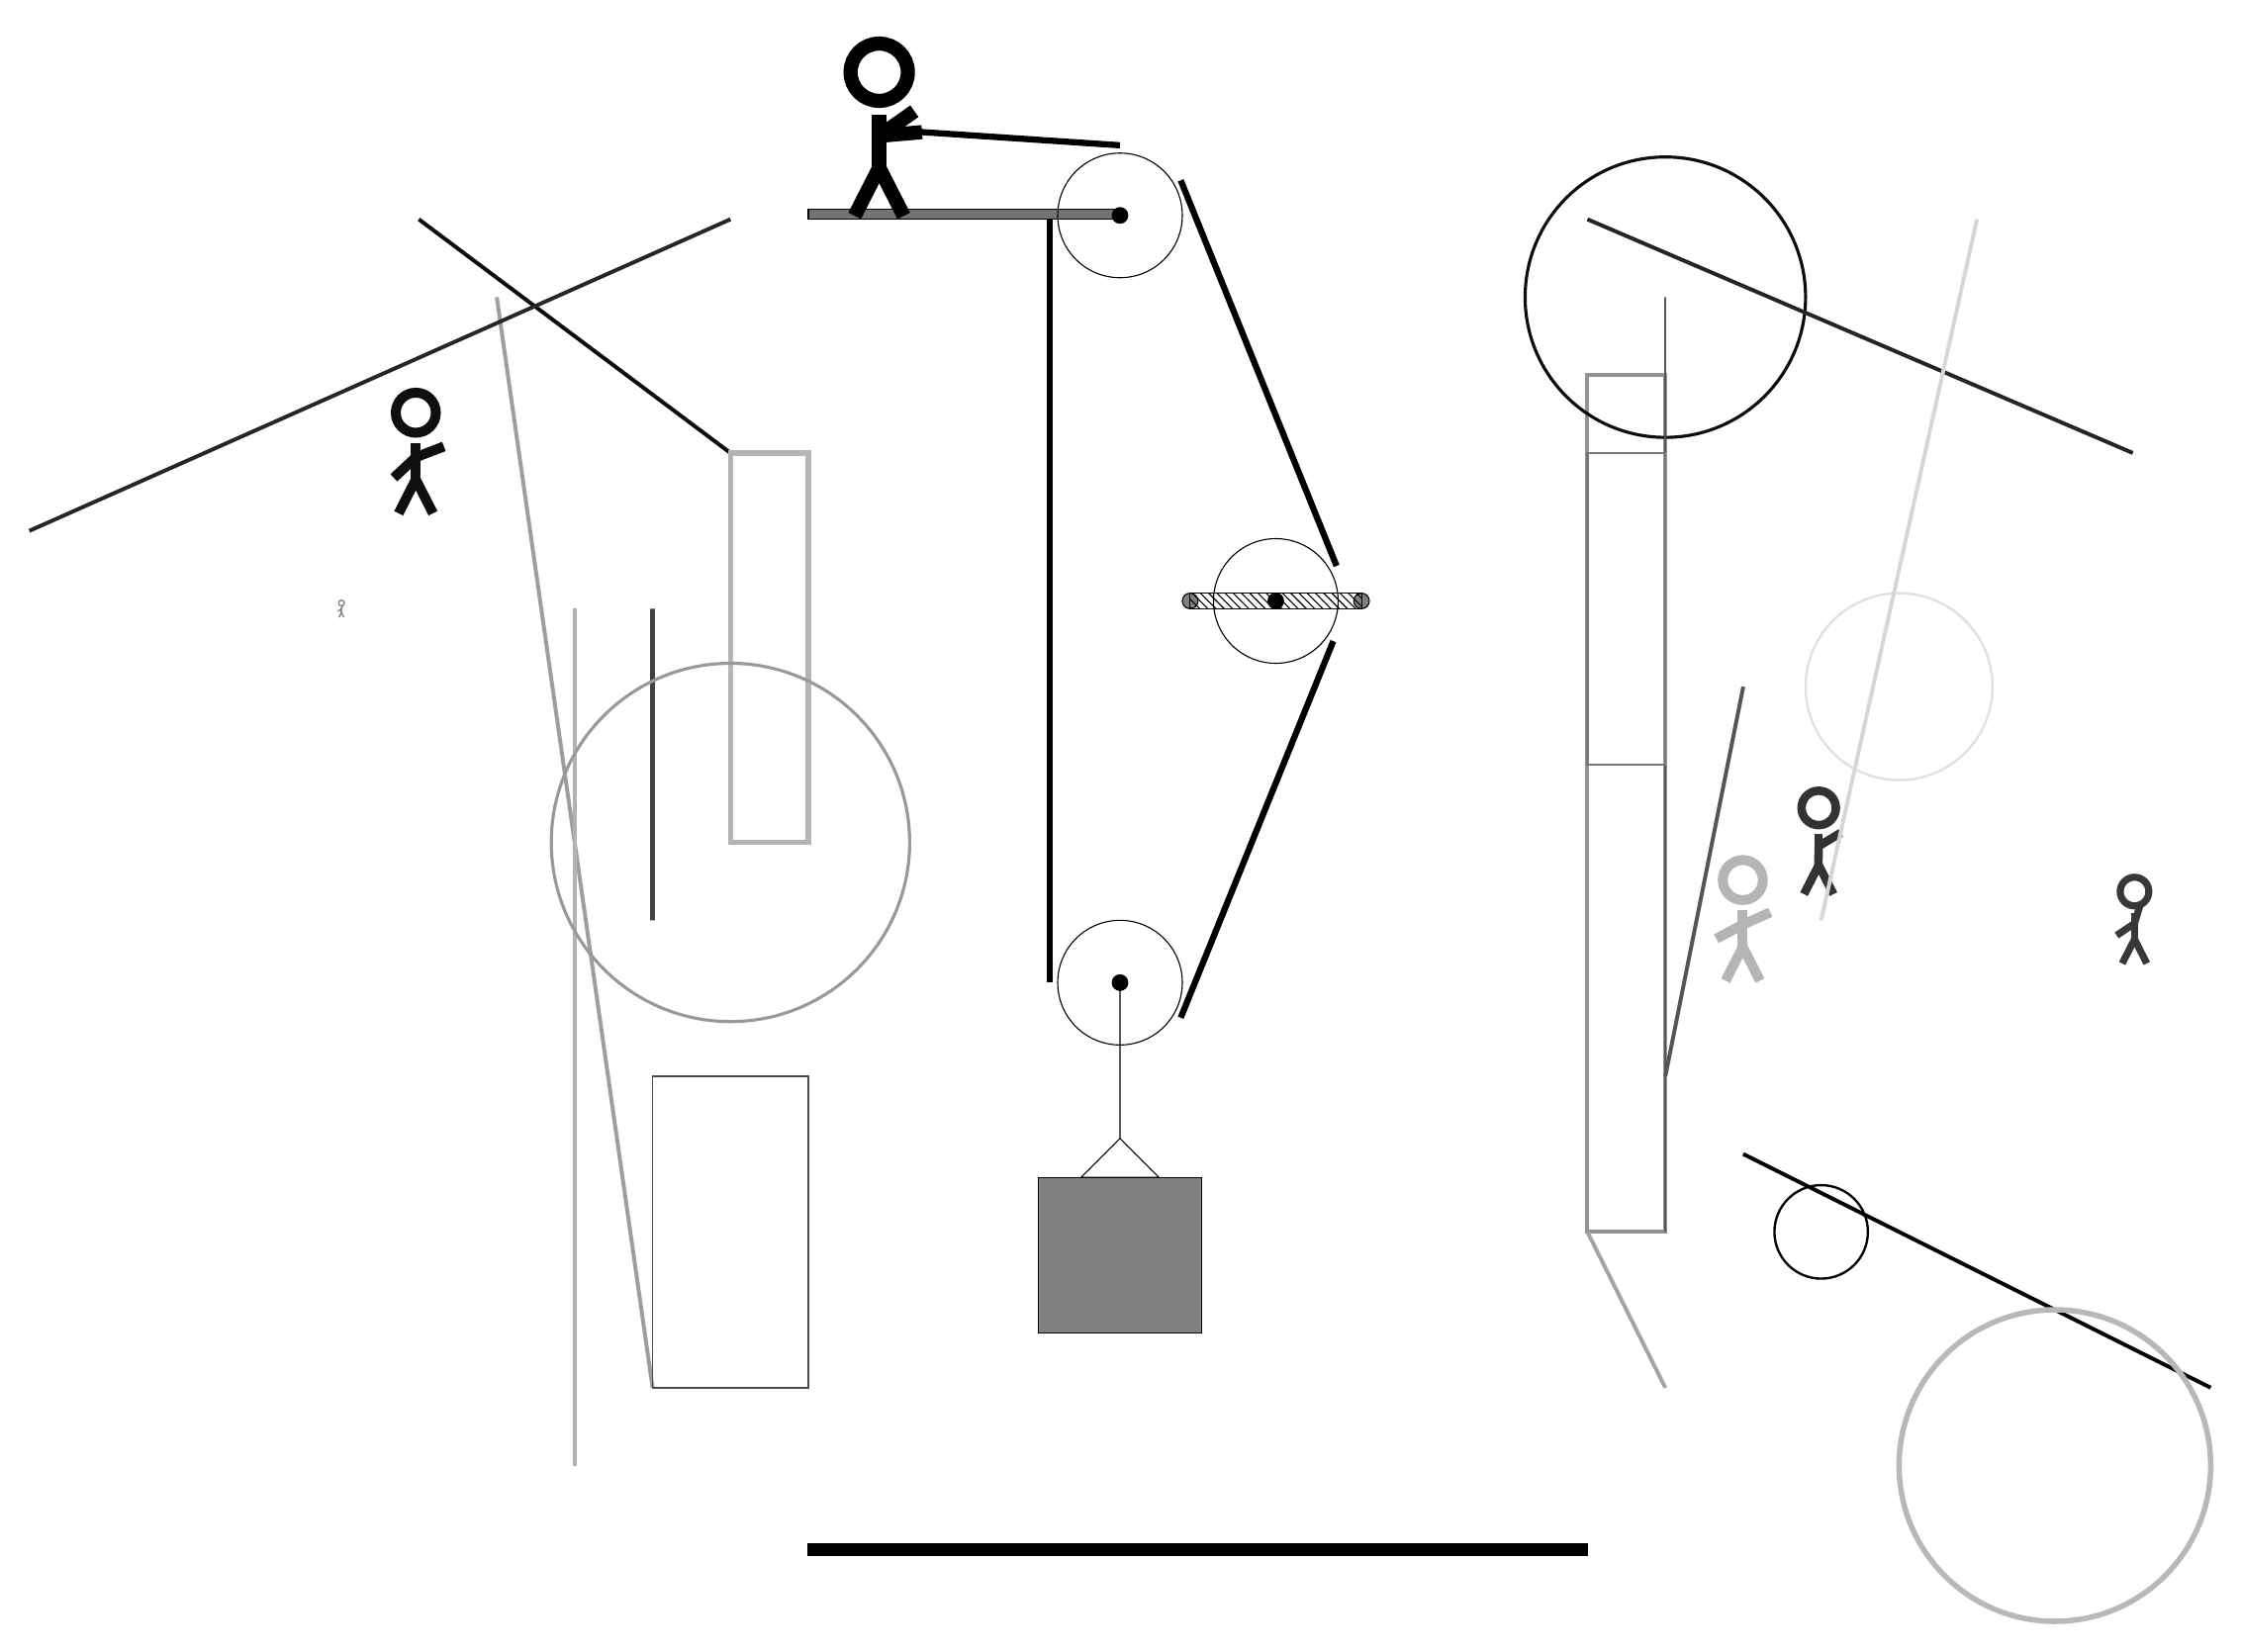
\begin{tikzpicture}
			%%%%% START %%%%%
			
			\draw[fill=black!55] (-2, 14) rectangle (2, 14.125);
			
			\draw (2, 4.2) circle (0.8);
			\draw[fill=black] (2, 4.2) circle (0.1);
			
			\draw (2, 14.05) circle (0.8);
			\draw[fill=black] (2, 14.05) circle (0.1);
			
			\draw[fill=white](4, 9.1) circle (0.8);
			\draw[fill=black] (4, 9.1) circle (0.1);
			\draw[fill=black!50] (2.9, 9.1) circle (0.1);
			\draw[fill=black!50] (5.1, 9.1) circle (0.1);
			\draw[pattern=north west lines, pattern color=black] (2.9, 9.2) rectangle (5.1, 9.0);
			
			\node[line width=0.4mm, color=black!80] at (11, 6) {\Strichmaxerl[6][89][31]};
			
			\draw[line width=0.5mm, color=black!38](-6, 13) -- (-4, -1);
			\draw[line width=0.7mm, color=black!74] (-4, 9) rectangle (-4, 5);
			\draw[line width=0.2mm, color=black!70] (-4, 3) rectangle (-2, -1);
			\draw[line width=0.5mm, color=black!95](-3, 11) -- (-7, 14);
			\draw[line width=0.5mm, color=black!85](-3, 14) -- (-12, 10);
			\draw[line width=0.7mm, color=black!29] (-2, 11) rectangle (-3, 6);
			
			\draw[line width=0.5mm, color=black!99](10, 2) -- (16, -1);
			\draw[line width=0.5mm, color=black!42] (9, 12) rectangle (8, 1);
			\draw[line width=0.5mm, color=black!61](11, 0) -- (11, 0);
			\draw [line width=0.4mm, color=black!95](9, 13) circle (1.8);
			
			\draw[line width=0.2mm, color=black!66] (9, 1) rectangle (9, 13);
			\node[line width=0.2mm, color=black!46] at (-8, 9) {\Strichmaxerl[1][24][74]};
			
			\draw [line width=0.3mm, color=black!99](11, 1) circle (0.6);
			\draw[line width=0.5mm, color=black!30](-5, 9) -- (-5, -2);
			\draw[line width=0.5mm, color=black!36](8, 1) -- (9, -1);
			\draw[line width=0.5mm, color=black!86](8, 14) -- (15, 11);
			\draw[line width=0.3mm, color=black!53] (9, 11) rectangle (8, 7);
			\node[line width=0.2mm, color=black!29] at (10, 5) {\Strichmaxerl[7][28][24]};
			\node[line width=0.7mm, color=black!94] at (-7, 11) {\Strichmaxerl[7][43][21]};
			\draw [line width=0.3mm, color=black!12](12, 8) circle (1.2);
			
			\draw[line width=0.5mm, color=black!67](9, 3) -- (10, 8);
			\draw [line width=0.4mm, color=black!40](-3, 6) circle (2.3);
			\draw[line width=0.5mm, color=black!16](13, 14) -- (11, 5);
			\draw [line width=0.7mm, color=black!28](14, -2) circle (2.0);
			
			\node[line width=0.6mm, color=black!78] at (15, 5) {\Strichmaxerl[5][34][73]};
			
			
			\draw (2, 4.2) -- (2, 2.2) -- (1.5, 1.7) -- (2.5, 1.7) -- (2, 2.2);
			\draw[fill=black!50] (0.95, 1.7) rectangle (3.05, -0.3);
			
			\draw[line width=0.8mm] (1.1, 14) -- (1.1, 4.2);
			\centerarc[line width=0.8mm](2, 4.2)(180:330:0.9);
			\draw[line width=0.8mm](2.7794, 3.75) -- (4.7373, 8.5838);
			\centerarc[line width=0.8mm](4, 9.1)(390:325:0.9);
			\draw[line width=0.8mm](4.7794, 9.55) -- (2.7794, 14.5);
			\centerarc[line width=0.8mm](2, 14.05)(30:90:0.9);
			\draw[line width=0.8mm](2, 14.95) -- (-1, 15.15);
			
			\node at (-1, 15.15) {\Strichmaxerl[10][-175][35]};
			
			\draw[fill=black] (-2, -3) rectangle (8, -3.15);
			
			%%%%% END %%%%%
		\end{tikzpicture}
	\end{figure}	
\end{document}